\section{Error Localisation Strategies}
\label{sec:background-localisation}

Section~\ref{sec:introduction-localisation} motivated a decomposition of the global DWR estimator into computable local contributions. Elementwise integration by parts (IBP) gives strong cell residuals, flux jumps, and boundary residuals, but its derivation depends on the differential operator and boundary conditions. Partition-of-unity (PU) localisation inserts functions \(\{\chi_i\}_{i=1}^M\), with \(\sum_i\chi_i=1\), into the weak residual and associates the resulting terms with basis functions or patches \cite{Richter_Wick_2015}. This is effective for stationary and space--time adaptivity \cite{ThieleWick2024,R6,non-flow}, but a single patch contribution may combine several residual mechanisms.

The present construction is indexed instead by geometric support. It separates cell-volume, spatial-facet, temporal-face, and, when present, mixed space--time ridge contributions. Polynomial densities on these entities are recovered directly from evaluations of the UFL weak residual in \texttt{Firedrake}, which does not require problem-specific strong residual or hand-derived flux-jump formula. This approach is motivated by the stationary bubble--cone construction of Rognes and Logg \cite{Rognes_Logg_2013}. We extend it below to discontinuous Galerkin discretisations in time.

% 我的直觉是切蛋糕 直接切割 - mathematically 边界部分就不见了（粘在刀上所以要刮到cell上），thats why ibp 或者 recovery 有必要；投影的话，边界部分不会受影响。
% 但是要怎么对比这个方法和投影呢？这个方法 more explainable？主要是感觉projection实在是快一些吗？


\subsection{Stationary Bubble and Cone Projection}
\label{sec:stationary-residual-recovery}

We first recall the stationary construction for the primal residual. The nonlinear adjoint-residual term is treated in Section~\ref{sec:nonlinear-adjoint-residual-localisation}. For each \(K\in\mathcal T_h\), let \(\mathcal F(K)\) denote its facets. Rognes and Logg formulate the following assumptinos \cite{Rognes_Logg_2013}:
\begin{description}
  \item[(A1) Global decomposition.] The global residual is a sum of cell-local functionals,
  \begin{equation}
    \rho(v)=\sum_{K\in\mathcal T_h}\rho_K(v).
    \label{eq:stationary-global-decomposition}
  \end{equation}

  \item[(A2) Local decomposition.] Each local residual has the form
  \begin{equation}
    \rho_K(v)
    =
    (R_K,v)_K
    +
    \sum_{F\in\mathcal F(K)}(R_{K,F},v)_F.
    \label{eq:stationary-residual-representation}
  \end{equation}

  \item[(A3) Polynomial representation.] The residual densities are piecewise polynomial. For chosen degrees \(p,q\),
  \begin{equation}
    R_K\in\mathbb P^p(K),
    \qquad
    R_{K,F}\in\mathbb P^q(F).
    \label{eq:stationary-polynomial-representability}
  \end{equation}
\end{description}
Assumptions (A1) and (A2) identify the residual-supporting entities, while (A3) determines whether the recovery is exact or a weighted projection.

For a \(d\)-simplex \(K\) with vertices \(\{v_i\}_{i=1}^{d+1}\) and associated barycentric coordinates \(\{\lambda_i^K\}_{i=1}^{d+1}\). The cell bubble is defined by 
\begin{equation}
  b_K:=\prod_{i=1}^{d+1}\lambda_i^K,
  \qquad b_K|_{\partial K}=0.
  \label{eq:recovery-cell-bubble}
\end{equation}
The bubble test eliminates all facet actions, so \(R_K^B\in\mathbb P^p(K)\) is recovered from
\begin{equation}
  (R_K^B,b_K\phi)_K
  =\rho_K(b_K\phi)
  \qquad\forall\phi\in\mathbb P^p(K).
  \label{eq:stationary-cell-projection}
\end{equation}

For \(F\in\mathcal F(K)\), let
\begin{equation}
  \mathcal I_F:=\{i:v_i\in F\},
  \qquad
  \beta_{K,F}:=\prod_{i\in\mathcal I_F}\lambda_i^K.
  \label{eq:recovery-facet-cone}
\end{equation}
This cone is nonzero on the relative interior of \(F\), vanishes on every other facet, and remains nonzero inside \(K\). Let
\begin{equation}
  E_{K,F}:\mathbb P^q(F)\longrightarrow\mathbb P^q(K),
  \qquad (E_{K,F}\psi)|_F=\psi,
  \label{eq:facet-polynomial-extension}
\end{equation}
and write \(\widetilde\psi=E_{K,F}\psi\). Once the cell density \(R_{K}^B\) is recovered, the facet resudual contribution \(R_{K,F}^B\in\mathbb P^q(F)\) is defined by
\begin{equation}
  \bigl(R_{K,F}^B,(\beta_{K,F}|_F)\psi\bigr)_F
  =
  \rho_K(\beta_{K,F}\widetilde\psi)
  -(R_K^B,\beta_{K,F}\widetilde\psi)_K
  \quad\forall\psi\in\mathbb P^q(F).
  \label{eq:stationary-facet-projection}
\end{equation}
The subtraction removes the cell action seen by the cone. Under (A1)--(A3), these weighted mass problems uniquely recover \(R_K\) and \(R_{K,F}\) \cite{Rognes_Logg_2013}.
Figure~\ref{fig:stationary-bubble-cone} illustrates the bubble and cone test functions used in the two stationary recovery problems.
\newcommand{\drawcoarsemeshdiagonals}{%
  \addplot3[gray!60, line width=0.25pt]
    coordinates {(0,0,0) (1,1,0)};
  \addplot3[gray!60, line width=0.25pt]
    coordinates {(0,.3333,0) (.6667,1,0)};
  \addplot3[gray!60, line width=0.25pt]
    coordinates {(0,.6667,0) (.3333,1,0)};
  \addplot3[gray!60, line width=0.25pt]
    coordinates {(.3333,0,0) (1,.6667,0)};
  \addplot3[gray!60, line width=0.25pt]
    coordinates {(.6667,0,0) (1,.3333,0)};
}
\vspace{1.6em}
\begin{figure}[h]
  \centering
    \begin{subfigure}[t]{0.48\textwidth}
    \centering
    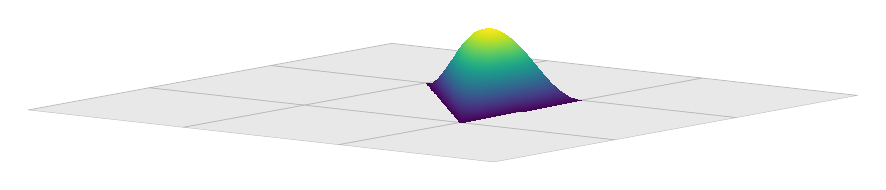
\begin{tikzpicture}
      \begin{axis}[
        width=\linewidth,
        height=5.2cm,
        view={-52}{27},
        axis lines=none,
        xmin=0, xmax=1,
        ymin=0, ymax=1,
        zmin=0, zmax=1,
        domain=0:1,
        y domain=0:1,
        samples=25,
        samples y=25,
        colormap/viridis
      ]
        % Coarse background mesh: 3-by-3 quadrilaterals, each divided into two triangles.
        \addplot3[
          surf,
          shader=flat,
          draw=gray!55,
          line width=0.25pt,
          fill=gray!18,
          domain=0:1,
          y domain=0:1,
          samples=4,
          samples y=4
        ] {0};
        \drawcoarsemeshdiagonals
        % One triangular element:
        % A = (1/3,1/3), B = (2/3,1/3), C = (2/3,2/3)
        % The factor 10.8 gives a displayed peak of about 0.4.
        \addplot3[
          surf,
          shader=interp,
          draw=none
        ]
        (
          {.3333 + .3334*x*(1-y) + .3334*y},
          {.3333 + .3334*y},
          {12*x*(1-x)*(1-y)^2*y}
        );
      \end{axis}
    \end{tikzpicture}

    \caption{Cell bubble \(b_K\).}
    \label{fig:stationary-cell-bubble}
  \end{subfigure}
  \hfill
  \begin{subfigure}[t]{0.48\textwidth}
    \centering
    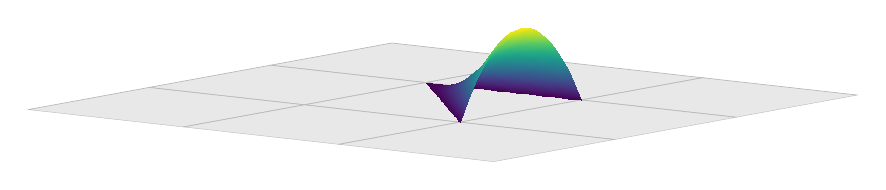
\begin{tikzpicture}
      \begin{axis}[
        width=\linewidth,
        height=5.2cm,
        view={-52}{27},
        axis lines=none,
        xmin=0, xmax=1,
        ymin=0, ymax=1,
        zmin=0, zmax=1,
        domain=0:1,
        y domain=0:1,
        samples=25,
        samples y=25,
        colormap/viridis
      ]
        \addplot3[
          surf,
          shader=flat,
          draw=gray!55,
          line width=0.25pt,
          fill=gray!18,
          domain=0:1,
          y domain=0:1,
          samples=4,
          samples y=4
        ] {0};
        \drawcoarsemeshdiagonals
        % Facet cone on the same triangular element.
        % The selected facet is AB: (1/3,1/3) -- (2/3,1/3).
        % The factor 1.6 gives a displayed peak of 0.4.
        \addplot3[
          surf,
          shader=interp,
          draw=none
        ]
        (
          {.3333 + .3334*x*(1-y) + .3334*y},
          {.3333 + .3334*y},
          {2*x*(1-x)*(1-y)^2}
        );

      \end{axis}
    \end{tikzpicture}

    \caption{Facet cone \(\beta_{K,F}\).}
    \label{fig:stationary-facet-cone}
  \end{subfigure}

  \caption{Bubble and cone test functions on a single triangular element \(K\).}
  \label{fig:stationary-bubble-cone}
\end{figure}

The recovered densities are paired with the computable dual weight \(z^\star\). The stationary analysis is established in \cite{Rognes_Logg_2013}, while the space--time extension below is assessed numerically in Chapter~\ref{chap:experiments} through localisation gaps, effectivities, and adaptive behaviour. The essential new feature is the dG action at each temporal interface.



\subsection{Space--Time Extension of the Residual Recovery}
\label{sec:space-time-residual-recovery}

Let \(V\) be a spatial trial and test space. We consider an abstract evolution problem of the form
\begin{equation}
  m(\partial_tu(t),v)+a(u(t);v,t)=\ell(v;t)
  \qquad\forall v\in V,\quad t\in(0,T),
  \label{eq:abstract-evolution-problem}
\end{equation}
with \(u(0)=u_0\). Here \(m\) is the time-derivative pairing, \(a\) contains the remaining spatial and possibly nonlinear terms, and \(\ell\) is the load. Let
\begin{equation}
  I_n=(t_{n-1},t_n],
  \qquad k_n=t_n-t_{n-1},
  \qquad Q_{K,n}=K\times I_n,
  \qquad \tau=\frac{t-t_{n-1}}{k_n}.
  \label{eq:space-time-cell}
\end{equation}
On \(I_n\), trial and test functions are time polynomials with values in a spatial finite-element space \(V_n\), and may be discontinuous at \(t_n\). Following the standard space--time dG notation \cite{Bangerth_Rannacher_2003}, define
\begin{equation}
  U^{n+}:=\lim_{t\downarrow t_n}U(t),
  \qquad
  U^{n-}:=\lim_{t\uparrow t_n}U(t),
  \qquad
  [U]^n:=U^{n+}-U^{n-}.
  \label{eq:dg-time-traces}
\end{equation}

For matching spatial spaces, the global dG semilinear form is
\begin{align}
  \mathcal A(U)(V)
  :={}&
  \sum_{n=1}^{N}\int_{I_n}
  \bigl[m(\partial_tU,V)+a(U;V,t)-\ell(V;t)\bigr],\mathrm dt
  \notag\\
  &+\sum_{n=2}^{N}m([U]^{n-1},V^{(n-1)+})
  +m(U^{0+}-u_0,V^{0+}).
  \label{eq:global-dg-semilinear-form}
\end{align}
The discrete problem is \(\mathcal A(U_h)(V_h)=0\) for all discrete tests. Throughout this chapter we use the convention
\begin{equation}
  \rho(U)(V):=-\mathcal A(U)(V).
  \label{eq:dg-residual-sign-convention}
\end{equation}

The extension of the stationary recovery is based on the following assumptions.

\begin{description}
  \item[(A1) Global decomposition.] The global residual is the sum of local space--time functionals,
  \begin{equation}
    \rho(U_h)(V)
    =
    \sum_{n=1}^{N}
    \sum_{K\in\mathcal T_n}
    \rho_{K,n}(U_h)(V).
    \label{eq:space-time-residual-decomposition}
  \end{equation}

To be more specific, we can define the incoming defect by
\begin{equation}
  \delta_{n-1}(U_h):=
  \begin{cases}
    U_h^{0+}-u_0, & n=1,\\[0.3em]
    [U_h]^{n-1}, & n>1.
  \end{cases}
  \label{eq:dg-incoming-defect}
\end{equation}
Thus
\begin{equation}
  \begin{aligned}
  \rho_{K,n}(U_h)(V)
  :={}&
  \int_{I_n}
  \Big[
    \ell_{K,n}(V;t)
    -
    m_{n,K}(\partial_tU_h,V)
    -
    a_{K,n}(U_h;V,t)
  \Big]\,\mathrm dt
  \\
  &-
  m_{n,K}\Big(
    \delta_{n-1}(U_h),
    V(t_{n-1}^{+})
  \Big).
  \end{aligned}
  \label{eq:complete-local-slab-residual}
\end{equation}

Note that if \(V_{n-1}\ne V_n\), the outgoing trace must first be transferred into \(V_n\):
\begin{equation}
  \delta_{n-1}(U_h)
  =U_h^{(n-1)+}-P_{n-1}U_h^{(n-1)-},
  \qquad n>1,
  \label{eq:transferred-dg-time-defect}
\end{equation}
where \(P_{n-1}:V_{n-1}\to V_n\). The transfer and its adjoint are discussed in Section~\ref{sec:slab-transfer-adjoint}.

  \item[(A2) Local decomposition.] On each space--time cell \(Q_{K,n}\), the residual admits a representation by contributions supported on the cell interior, spatial facets, temporal facets, and, when required by the chosen pairing, their intersections, as shown in Figure~\ref{fig:space-time-residual-entities}.
  \begin{equation}
    \begin{aligned}
    \rho_{K,n}(U_h)(V)
    ={}&
    (R_{K,n}^{B,\mathrm{vol}},V)_{Q_{K,n}}
    +
    \sum_{F\subset\partial K}
    (R_{K,F,n}^{B,\mathrm{sf}},V)_{F\times I_n}
    \\
    &+
    (R_{K,n-1}^{B,\mathrm{tf}},V(t_{n-1}^{+}))_{K} +
    \sum_{F\subset\partial K}
    (R_{F,n-1}^{B,\mathrm{xt}},
      V(t_{n-1}^{+}))_{F}.
    \end{aligned}
    \label{eq:space-time-entity-representation}
  \end{equation}

\begin{figure}[h]
  \centering
  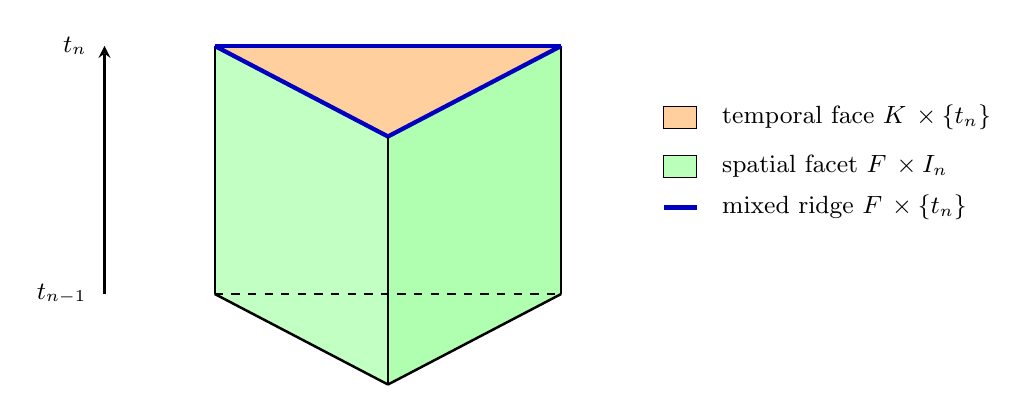
\begin{tikzpicture}[
    x=1cm,y=1cm,>=stealth,font=\small,
    edge/.style={black,line width=.9pt},
    hidden edge/.style={black,dashed,line width=.9pt},
    temporal/.style={fill=orange!38},
    spatial/.style={fill=green!24},
    ridge/.style={blue!75!black,line width=1.55pt},
    hidden ridge/.style={blue!65!black,dashed,line width=1.3pt}
  ]
    % The prism is viewed from its incoming temporal face.
    \coordinate (A)  at (2.55,0);
    \coordinate (B)  at (.35,1.15);
    \coordinate (C)  at (4.75,1.15);
    \coordinate (At) at (2.55,3.15);
    \coordinate (Bt) at (.35,4.30);
    \coordinate (Ct) at (4.75,4.30);

    % The two spatial facets recede from the incoming face.
    \fill[spatial] (A)--(B)--(Bt)--(At)--cycle;
    \fill[green!31] (A)--(C)--(Ct)--(At)--cycle;

    % The incoming face is nearest to the reader and therefore overlays
    % the projected lower portions of the spatial facets.
    % \fill[temporal] (A)--(B)--(C)--cycle;
    % Outgoing temporal face K x {t_n}
    \fill[temporal] (At)--(Bt)--(Ct)--cycle;

    % Ordinary space--time edges.  The central edge faces the reader.
    \draw[edge] (A)--(At);
    \draw[edge] (B)--(Bt);
    \draw[edge] (C)--(Ct);

    % The three incoming mixed ridges are all visible.
    \draw[edge] (A)--(B);
    \draw[edge] (A)--(C);
    \draw[hidden edge] (B)--(C);

    % Two outgoing ridges are visible; the rear ridge is hidden.
    \draw[ridge] (At)--(Bt);
    \draw[ridge] (At)--(Ct);
    \draw[ridge] (Bt)--(Ct);

    % Time direction: from the near incoming face to the remote face.
    \draw[->,line width=.9pt] (-1.05,1.15)--(-1.05,4.30);
    \node[left=3pt] at (-1.05,1.15) {\(t_{n-1}\)};
    \node[left=3pt] at (-1.05,4.30) {\(t_n\)};

    % \node[below=4pt,align=center] at (A)
    %   {incoming temporal face\\[-1pt]\(K\times\{t_{n-1}\}\)};
    % \node[above=4pt,align=center] at (2.55,4.30)
    %   {outgoing temporal face\\[-1pt]\(K\times\{t_n\}\)};
    % \node[rotate=18,align=center] at (1.35,2.25)
    %   {spatial facet\\[-1pt]\(F_1\times I_n\)};
    % \node[rotate=-18,align=center] at (3.75,2.25)
    %   {spatial facet\\[-1pt]\(F_2\times I_n\)};

    \begin{scope}[xshift=6.05cm,yshift=3.25cm]
      \fill[orange!38] (0,0) rectangle (.42,.28);
      \draw[black,thin] (0,0) rectangle (.42,.28);
      \node[anchor=west] at (.62,.14) {temporal face $K\,\times \{t_n\}$};
      \fill[green!27] (0,-.62) rectangle (.42,-.34);
      \draw[black,thin] (0,-.62) rectangle (.42,-.34);
      \node[anchor=west] at (.62,-.48) {spatial facet $F\,\times I_n$};
      \draw[ridge] (0,-1.00)--(.42,-1.00);
      \node[anchor=west] at (.62,-1.00) {mixed ridge $F\,\times \{t_n\}$};
      % \draw[hidden ridge] (0,-1.46)--(.42,-1.46);
      % \node[anchor=west] at (.62,-1.46) {hidden mixed ridge};
    \end{scope}
  \end{tikzpicture}
  \caption{Space--time cell \(Q_{K,n}=K\times I_n\).}
  \label{fig:space-time-residual-entities}
\end{figure}

  
\item[(A3) Polynomial representation.]
The residual densities belong to the selected recovery spaces,
\begin{align}
  R_{K,n}^{\mathrm{vol}}
  &\in Q_{K,n}^{p_x,p_t},
  &
  R_{K,F,n}^{\mathrm{sf}}
  &\in Q_{F,n}^{q_x,q_t},
  \notag\\
  R_{K,n-1}^{\mathrm{tf}}
  &\in \mathbb P^{r_x}(K),
  &
  R_{K,F,n-1}^{\mathrm{xt}}
  &\in \mathbb P^{s_x}(F),
  \label{eq:space-time-polynomial-representability}
\end{align}
whenever the corresponding densities are present.
\end{description}

Assumption (A1) follows naturally when the weak form is assembled slab by slab from cell and facet integrals. (A2) records the geometric supports. Under (A3), problems recover a density exactly when it belongs to the selected polynomial space.


\paragraph{Volume recovery.}
We define the temporal interior bubble and its tensor product with the spatial cell bubble from~\cref{eq:recovery-cell-bubble} by
\begin{equation}
  b_n^t(\tau):=4\tau(1-\tau),
  \qquad
  B_{K,n}:=b_Kb_n^t.
  \label{eq:space-time-volume-bubble}
\end{equation}
The function \(B_{K,n}\) vanishes on every codimension-one face of \(Q_{K,n}\). In particular,
\[
  B_{K,n}(t_{n-1}^{+})
  =
  B_{K,n}(t_n^{-})
  =
  0,
\]
so the temporal-interface term in \cref{eq:complete-local-slab-residual} vanishes under this test.

The recovered volume density \(R_{K,n}^{B,\mathrm{vol}}\in Q_{K,n}^{p_x,p_t}\) is defined by
\begin{equation}
  \bigl(
    R_{K,n}^{B,\mathrm{vol}},
    B_{K,n}\Phi
  \bigr)_{Q_{K,n}}
  =
  \rho_{K,n}(U_h)\bigl(B_{K,n}\Phi\bigr)
  \qquad
  \forall\Phi\in Q_{K,n}^{p_x,p_t}.
  \label{eq:space-time-volume-projection}
\end{equation}
All spatial-facet and temporal-endpoint contributions vanish under this test.

\paragraph{Spatial-facet recovery.}
For \(F\subset\partial K\), define
\begin{equation}
  C_{K,F,n}^{\mathrm{sf}}
  :=
  \beta_{K,F}b_n^t.
  \label{eq:space-time-spatial-cone}
\end{equation}

Let
\(
  E_{K,F,n}:
  Q_{F,n}^{q_x,q_t}
  \longrightarrow
  Q_{K,n}^{q_x,q_t}
\)
be a fixed polynomial extension and write \(\widetilde\Psi:=E_{K,F,n}\Psi\). After the volume density has been recovered, we can define \(R_{K,F,n}^{B,\mathrm{sf}}\in Q_{F,n}^{q_x,q_t}\) by
\begin{align}
  &\Bigl(
    R_{K,F,n}^{B,\mathrm{sf}},
    \bigl.C_{K,F,n}^{\mathrm{sf}}\bigr|_{F\times I_n}\Psi
  \Bigr)_{F\times I_n}
  \notag\\
  &\qquad =
  \rho_{K,n}(U_h)
  \bigl(C_{K,F,n}^{\mathrm{sf}}\widetilde\Psi\bigr)
  -
  \Bigl(
    R_{K,n}^{B,\mathrm{vol}},
    C_{K,F,n}^{\mathrm{sf}}\widetilde\Psi
  \Bigr)_{Q_{K,n}}
  \notag
  \qquad \quad
  \forall\Psi\in Q_{F,n}^{q_x,q_t}.
  \label{eq:space-time-spatial-facet-projection}
\end{align}


\paragraph{Temporal-face recovery.}
To isolate the incoming dG interface contribution, we define
\begin{equation}
  C_{K,n}^{\mathrm{tf},-}
  :=
  b_K(1-\tau),
  \label{eq:temporal-trace-cone}
\end{equation}
which satisfies
\begin{equation*}
  C_{K,n}^{\mathrm{tf},-}(t_{n-1}^{+})=b_K,
  \qquad
  C_{K,n}^{\mathrm{tf},-}(t_n^{-})=0,
  \qquad
  \left.C_{K,n}^{\mathrm{tf},-}\right|_{\partial K\times I_n}=0.
  \label{eq:temporal-cone-traces}
\end{equation*}

For \(\chi\in\mathbb P^{r_x}(K)\), we define
\begin{equation}
  \mathcal E_{K,n}^{\mathrm{tf}}(\chi)
  :=
  b_K(1-\tau)\chi.
  \label{eq:temporal-recovery-test}
\end{equation}
Since \(b_K|_{\partial K}=0\), this test has no trace on any spatial facet. Applying to the decomposition of the local residual gives
\begin{equation}
  \rho_{K,n}(U_h)
  \bigl(\mathcal E_{K,n}^{\mathrm{tf}}(\chi)\bigr)
  =
  \Bigl(
    R_{K,n}^{\mathrm{vol}},
    \mathcal E_{K,n}^{\mathrm{tf}}(\chi)
  \Bigr)_{Q_{K,n}}
  +
  \bigl(
    R_{K,n-1}^{\mathrm{tf}},
    b_K\chi
  \bigr)_K.
  \label{eq:temporal-cone-support-splitting}
\end{equation}
Thus the test exposes only the slab-volume residual and the incoming temporal-face residual. After recovering the volume density, we can determine \(R_{K,n-1}^{B,\mathrm{tf}}\in\mathbb P^{r_x}(K)\) from
\begin{equation}
  \begin{aligned}
  \bigl(
    R_{K,n-1}^{B,\mathrm{tf}},
    b_K\chi
  \bigr)_K
  ={}&
  \rho_{K,n}(U_h)
  \bigl(\mathcal E_{K,n}^{\mathrm{tf}}(\chi)\bigr)
  \\
  &-
  \Bigl(
    R_{K,n}^{B,\mathrm{vol}},
    \mathcal E_{K,n}^{\mathrm{tf}}(\chi)
  \Bigr)_{Q_{K,n}},
  \qquad
  \forall\chi\in\mathbb P^{r_x}(K).
  \end{aligned}
  \label{eq:temporal-facet-projection}
\end{equation}

% Assuming exact volume recovery on the chosen test space, the temporal density is determined by
% \begin{equation}
%   \bigl(
%     R_{K,n-1}^{B,\mathrm{tf}},
%     b_K\chi
%   \bigr)_K
%   =
%   -
%   m_{n,K}\bigl(
%     \delta_{n-1}(U_h),
%     b_K\chi
%   \bigr),
%   \qquad
%   \forall\chi\in\mathbb P^{r_x}(K).
% \end{equation}
% For the standard \(L^2(K)\) mass pairing, this is the \(b_K\)-weighted projection of \(-\delta_{n-1}(U_h)\).


\paragraph{Possible mixed spatial--temporal ridge.}
A separate mixed recovery is required only if the complete residual contains a nonzero functional supported on \(F\times\{t_{n-1}\}\). Such a contribution does not normally arise from an \(L^2\) time-mass pairing, but it can occur when the pairing contains spatial derivatives, as discussed for the BBM problem in Section~\ref{sec:bbm-mixed-ridge-specialisation}.

For \(\psi\in\mathbb P^{s_x}(F)\), let \(\widetilde\psi=E_{K,F}\psi\) be the fixed extension used in the stationary facet recovery and define
\begin{equation}
  \begin{aligned}
  C_{K,F,n}^{\mathrm{xt},-}
  &:=
  \beta_{K,F}(1-\tau),
  \\
  \mathcal{E}_{K,F,n}^{\mathrm{xt}}(\psi)
  &:=
  C_{K,F,n}^{\mathrm{xt},-}\widetilde\psi.
  \end{aligned}
  \label{eq:mixed-ridge-test}
\end{equation}
% This test is nonzero in the slab interior, on the selected spatial facet, and on the left temporal face. 
The mixed density \(R_{K,F,n-1}^{B,\mathrm{xt}}\in\mathbb P^{s_x}(F)\) is consequently defined by
\begin{align}
  \bigl(
    R_{K,F,n-1}^{B,\mathrm{xt}},
    (\beta_{K,F}|_F)\psi
  \bigr)_F &=
  \rho_{K,n}(U_h)
  \bigl(\mathcal{E}_{K,F,n}^{\mathrm{xt}}(\psi)\bigr)
  -
  \Bigl(
    R_{K,n}^{B,\mathrm{vol}},
    \mathcal{E}_{K,F,n}^{\mathrm{xt}}(\psi)
  \Bigr)_{Q_{K,n}}
  \notag\\
  &-
  \Bigl(
    R_{K,F,n}^{B,\mathrm{sf}},
    \left.\mathcal{E}_{K,F,n}^{\mathrm{xt}}(\psi)\right|_{F\times I_n}
  \Bigr)_{F\times I_n}
  \notag\\
  &-
  \Bigl(
    R_{K,n-1}^{B,\mathrm{tf}},
    \mathcal{E}_{K,F,n}^{\mathrm{xt}}(\psi)(t_{n-1}^{+})
  \Bigr)_K,
  \qquad
  \forall\psi\in\mathbb P^{s_x}(F).
  \label{eq:mixed-ridge-recovery}
\end{align}
This subtraction leaves only the contribution supported on \(F\times\{t_{n-1}\}\).


\subsection{Localisation of the Nonlinear Adjoint-Residual Term}
\label{sec:nonlinear-adjoint-residual-localisation}

The construction above isolates the primal residual. For the nonlinear identity, the implemented estimator is
\begin{equation}
 \eta
 =
 \frac12\rho(u_h)(z_h^+-z_h)
 +\frac12\rho^\ast(u_h,z_h)(u_h^+-u_h)
 -\rho(u_h)(z_h),
 \label{eq:symmetric-nonlinear-dwr}
\end{equation}
with the unknown cubic remainder omitted. For the adjoint-residual term \(\rho^\ast(u_h,z_h)(u_h^+-u_h)\). Once \(u_h\) and \(z_h\) are fixed, \(\rho^\ast(u_h,z_h)\) is a linear functional of the primal variation. Consequently, the same bubble--cone principle can be applied to this term, but it requires a separate recovery of the linearised PDE and goal derivatives rather than reuse of the primal-residual densities.

In the present implementation, this second hierarchical recovery is not performed. Instead, the adjoint-residual action is assembled directly against discontinuous cellwise-constant test functions. Since the DG0 cell characteristic functions sum to one, this produces an algebraically closing cellwise partition of the assembled weak action. 
The resulting cell contributions are used together with the recovered primal-residual and Galerkin-correction terms in the nonlinear indicator. A complete bubble--cone recovery of \(\rho^\ast\) remains a possible extension when a separate entity-resolved interpretation of the adjoint-residual term is required.



\subsection{Localisation Diagnostics and Scope}

Let
\begin{equation}
 \eta_{\mathrm{loc}}:=\sum_{n,K}\eta_{K,n},
 \qquad
 \delta_{\mathrm{loc}}
 :=\eta_{\mathrm{loc}}-\eta_{\mathrm{glob}}.
 \label{eq:localisation-gap}
\end{equation}
The code records the signed gap, its relative value \(|\delta_{\mathrm{loc}}|/\max(|\eta_{\mathrm{glob}}|,\epsilon_{\mathrm{mach}})\), 
and the closure ratio \(\eta_{\mathrm{loc}}/\eta_{\mathrm{glob}}\). These quantities test whether the entity recovery reproduces the independently assembled weak estimator. They are distinct from effectivity, which compares an estimator with the true goal error and therefore also tests the enriched primal--dual approximation.

The construction requires a local finite-order weak residual, inclusion of all physical and discretisation terms, and stable weighted mass systems. Conforming scalar \(H^1\) problems fit this description directly. Discontinuous, \(H(\mathrm{div})\), and \(H(\mathrm{curl})\) formulations require recovery spaces that respect their numerical fluxes and normal or tangential traces. Saddle-point systems, variational inequalities, nonlocal operators, shocks, and distributional sources may require additional problem-specific support entities.

